\documentclass[pdfa,cucitura]{toptesi}
\hypersetup{%
	pdfpagemode={UseOutlines},
	bookmarksopen,
	pdfstartview={FitH},
	colorlinks,
	linkcolor={blue},
	citecolor={red},
	urlcolor={blue}
}

\usepackage[latin1]{inputenc}

% exact placing figures
\usepackage{float}

% insert eps files
\usepackage{epstopdf}

% cool tables
\usepackage{booktabs}
\usepackage{rotating}

\usepackage{mathrsfs}
\usepackage{amsmath}

\usepackage{caption}

\selectlanguage{english}

\ateneo{Politecnico di Torino}
\titolo{Building Trustworthiness Into Marketplaces}

\corsodilaurea{Computer Engineering}

\candidato{Marco \textsc{Terrinoni}}
\relatore{prof.\ Antonio Lioy}
%\tutoreaziendale{Stuart Short}

\sedutadilaurea{\textsc{Anno~accademico} 2013-2014}
\logosede{img/logopolito}

% per inserire uno spazio "fantasma" nella definizione di un'abbreviazione
\usepackage{xspace}

% per inserire un DOI senza problemi coi caratteri "strani" ivi presenti
\usepackage{doi}
\renewcommand{\doitext}{DOI }% originally was "doi:"

% per inserire correttamente le unit� di misura SI (incluse quelle binarie)
\usepackage[binary-units]{siunitx}
% se si desidera usare / invece che la potenza -1 per indicare "al secondo"
\sisetup{per-mode=symbol}

% per inserire codice di programmazione complesso
\usepackage{listings}% per inserire codice di programmazione complesso
\lstset{
basicstyle=\ttfamily,
columns=fullflexible,
xleftmargin=3ex,
breaklines,
breakatwhitespace,
escapechar=`
}

% modify some page parameters
\setlength{\parskip}{\medskipamount}
\advance\voffset -5mm
\advance\textheight 30mm

% riga orizzontale
\newcommand{\HRule}{\rule{\linewidth}{0.2mm}}
% esempio di creazione di semplici abbreviazioni
\newcommand{\ltx}{\LaTeX\xspace}
\newcommand{\txw}{TeXworks\xspace}
\newcommand{\mik}{MikTex\xspace}
\newcommand{\html}{HTML\xspace}
\newcommand{\xhtml}{XHTML\xspace}
\newcommand*\rot{\rotatebox{90}}

\newcommand{\latex}{\LaTeX\xspace}

% esempio di creazione di un'abbreviazione con un parametro (il cui uso � indicato da #1)
\newcommand{\cmd}[1]{\texttt{#1}\xspace}
% per citare un RFC, es. \rfc{822}
\newcommand{\rfc}[1]{RFC-#1\xspace}
% per citare un file (es. \file{autoexec.bat}) o una URI fittizia (es. \file{http://www.lioy.it/})
% per le URI vere usare \url o \href
\newcommand{\file}[1]{\texttt{#1}\xspace}
% per inserire codice di esempio in-line
\newcommand{\code}[1]{\lstinline|#1|}
% importante per i pathname Windows perch� non si pu� usare \ essendo un carattere riservato di Latex
\newcommand{\bs}{\textbackslash}
% definizione di un termine: formattazione ed inserimento nell'indice
\newcommand{\tdef}[1]{\textit{#1}\index{#1}}
% meta-termine, usato tipicamente nelle definizioni dei tag
\newcommand{\meta}[1]{\textit{#1}}

\begin{document}
\english

\errorcontextlines=9

\expandafter\ifx\csname StileTrieste\endcsname\relax
%\frontespizio
\else
	\paginavuota
	\begin{dedica}
		To my grandparents

		\textdagger\ You will always live in my memories
	\end{dedica}
	\tomo
\fi

\sommario
This document collects the various personal notes from the course ``Formal Languages and Compilers'' (2012), prof. Silvano Rivoira.
The \latex source code is available in a dedicated \href{https://github.com/terrinoni/FormalLanguagesAndCompilers-Notes}{GitHub repository}.

\indici

\mainmatter

\part{Formal Languages}

\chapter{Classification (FLC)}
\section{Grammars}
A grammar is a 4-tuple $G = (N, T, P, S)$ where:
\begin{description}
	\item[$N:$] alphabet of \underline{non-terminal} symbols;
	\item[$T:$] alphabet of \underline{terminal} symbols:
	\begin{itemize}
		\item $N \cap T = 0$ (two alphabets are disjoined),
		\item $V = N \cup T$ (alphabet of the grammar);
	\end{itemize}
	\item[$P:$] finite set of rules (productions);
	\item[$S:$] start (non-terminal) symbol.
\end{description}

A language produced by $G = (N, T, P, S)$ is:
$$
	L(G) = \left\{w \middle| w \in T^\ast; S \Rightarrow^\ast w\right\}
$$
Grammars that produce the same languages are said ``equivalent''.

\subsection{Types of Grammars}
\begin{description}
	\item[Type 0 grammars] (phase-structure)
		$$
			P = \left\{\alpha \to \beta \middle| \alpha \in V^+; \alpha \notin T^+; \beta \in V^\ast \right\}
		$$
	\item[Type 1 grammars] (context-sensitive)
		$$
			P = \left\{\alpha \to \beta \middle| \alpha \in V^+; \alpha \notin T^+; \beta \in V^+; |\alpha| \leq |\beta| \right\}
		$$
	\item[Type 2 grammars] (context-free)
		$$
			P = \left\{A \to \beta \middle| A \in N; \beta \in V^+ \right\}
		$$
\end{description}

\subsection{Linear Grammars}
$$
	P = \left\{A \to xBy, A \to x \middle| A, B \in N; x,y \in T^+ \right\}
$$
\begin{description}
	\item[Type 3 grammars] (right/left - linear)
	\begin{itemize}
		\item Right-Linear grammars
			$$
				P = \left\{A \to xB, A \to x \middle| A, B \in N; x \in T^+ \right\}
			$$
		\item Left-Linear grammars
			$$
				P = \left\{A \to Bx, A \to x \middle| A, B \in N; x \in T^+ \right\}
			$$
	\end{itemize}
	\item[Type 3 grammars] (right/left - regular)
	\begin{itemize}
		\item Right-Regular grammars
			$$
				P = \left\{A \to aB, A \to a \middle| A, B \in N; a \in T \right\}
			$$
		\item Left-Regular grammars
			$$
				P = \left\{A \to Ba, A \to a \middle| A, B \in N; a \in T \right\}
			$$
	\end{itemize}
\end{description}

\chapter{Regular Languages (RL)}
\section{Deterministic Finite Automata (DFA)}
A DFA is a 5-tuple $A = (Q, \Sigma, \delta, q_0, F)$ where:
\begin{description}
	\item[$Q:$] finite (non-empty) set of states;
	\item[$\Sigma:$] alphabet of input symbols;
	\item[$\delta:$] transition function:
		$$
			\delta: Q \times \Sigma \to Q
		$$
	\item[$q_0:$] start state:
		$$
			q_0 \in Q
		$$
	\item[$F:$] set of final states:
		$$
			F \subseteq Q
		$$
\end{description}

\subsection{Transition Table}
Transitional Table is a tabular representation of this transition function.

\subsection{Transition Diagram}
Transitional Diagram is a graph where:
\begin{itemize}
	\item for each state in the automaton there a node;
	\item for each transition $\delta(p, a) = q$ there is an arc from $p$ to $q$ labelled $a$.
\end{itemize}
The start state has an entering non-labelled arc and the final states are marked by a double circle.

\section{Non-Deterministic Finite Automata (NFA)}
An NFA is a 5-tuple $A = (Q, \Sigma, \delta, q_0, F)$ where:
\begin{description}
	\item[$Q:$] finite (non-empty) set of states;
	\item[$\Sigma:$] alphabet of input symbols;
	\item[$\delta:$] transition function:
		$$
			\delta: Q \times \Sigma \to \mathscr{P}(Q)
		$$
		$\mathscr{P}(Q)$: powerset of Q (the set of all subsets)
		$$
			\|\mathscr{P}(Q)\| = 2^{\|Q\|}
		$$
	\item[$q_0:$] start state:
		$$
			q_0 \in Q
		$$
	\item[$F:$] set of final states:
		$$
			F \subseteq Q
		$$
\end{description}
NB: a DFA is a special case of NFA.

\section{Equivalence of NFA and DFA}
\begin{figure}[H]
    \centerline{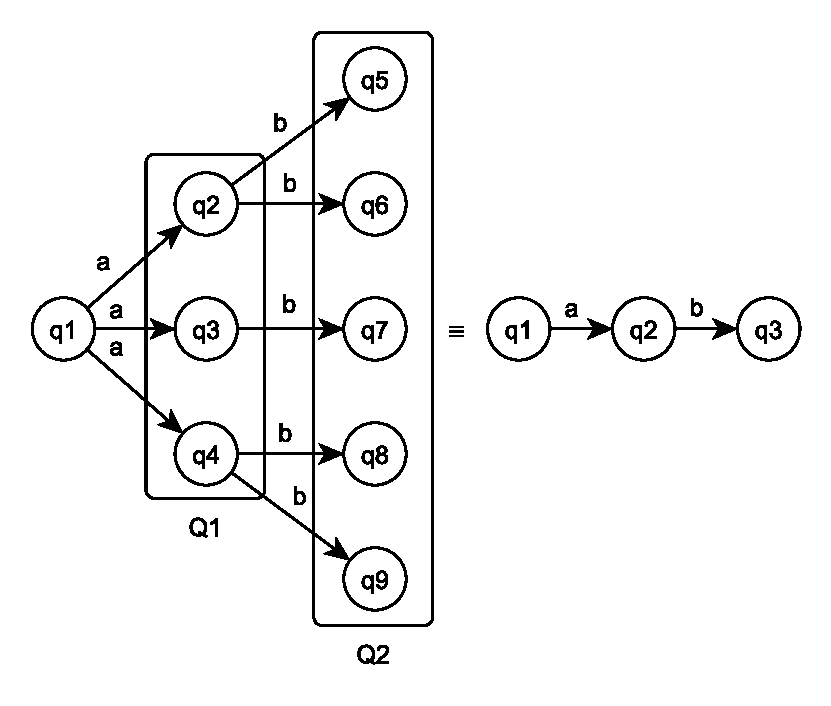
\includegraphics[width=0.6\textwidth]{img/1.pdf}}
\end{figure}
\begin{align*}
	Q_1 &= \left\{q_2, q_3, q_4\right\}\\
	Q_2 &= \left\{q_5, q_6, q_7, q_8, q_9\right\}
\end{align*}

Let $N = (Q_n, \Sigma, \delta_n, q_0, F_n)$ be an NFA; let us construct a DFA $D = (Q_d, \Sigma, \delta_d, \left\{q_0\right\}, F_d)$ where:
\begin{itemize}
	\item $Q_d \subseteq \mathscr{P}(Q_n)$;
	\item $\delta_d(S, a) = \cup_i \delta_n(p_1, a)$ where $p_i \in S \in Q_d$;
	\item $F_d = \left\{S \middle| S \in Q_d; S \cap F_n \neq \emptyset \right\}$.
\end{itemize}
By construction $L(D) = L(N)$, so $NFA \equiv DFA$

\section{From Finite Automata to Regular Expression}
It is possible to eliminate states in a Finite Automata by maintaining all the paths and by labelling the transitions with regular expressions:
\begin{figure}[H]
	\centerline{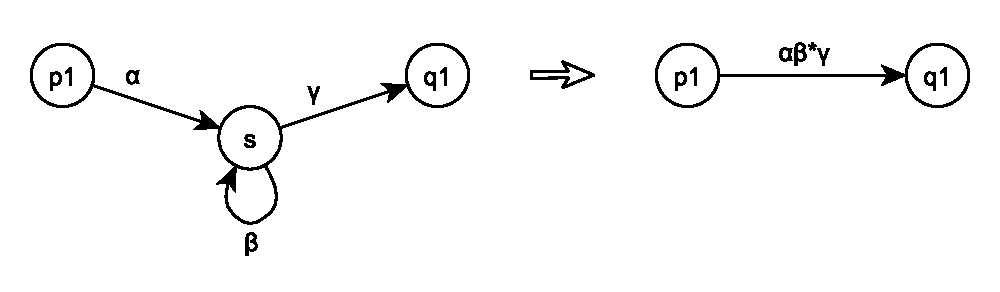
\includegraphics[width=0.7\textwidth]{img/2.pdf}}
\end{figure}
Given a finite state automaton $FA = (Q, \Sigma, \delta, q_0, F)$, add an initial state $A$ and a final state $\Omega$:
\begin{figure}[H]
	\centerline{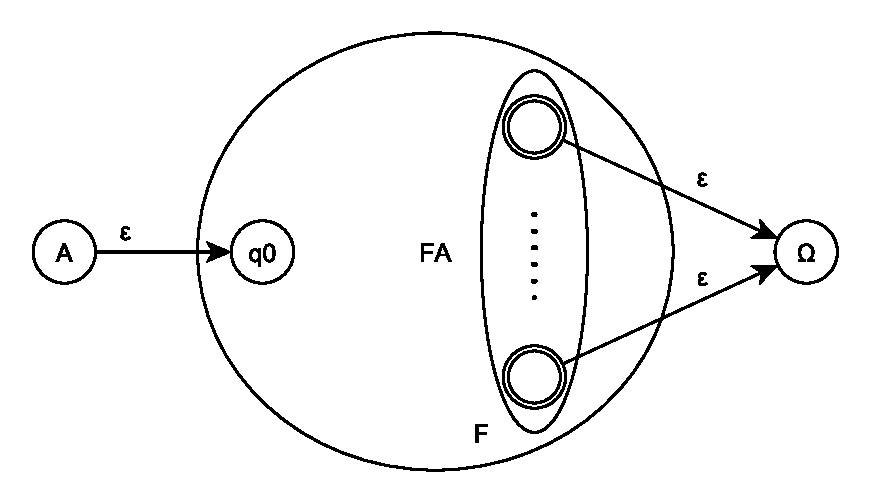
\includegraphics[width=0.7\textwidth]{img/3.pdf}}
\end{figure}
\begin{itemize}
	\item eliminate all the states in $FA$;
	\item the union of the labels on the transitions from $A$ to $\Omega$ gives the regular expression of the language $L(FA)$.
\end{itemize}

\section{From Regular Expression to Finite Automata}

\subsection{Regular Sets}
The regular sets: $0$, $\left\{\varepsilon\right\}$, $\left\{a\right\}$, $a \in \Sigma$ are accepted by finite state automata.
\begin{figure}[H]
	\centerline{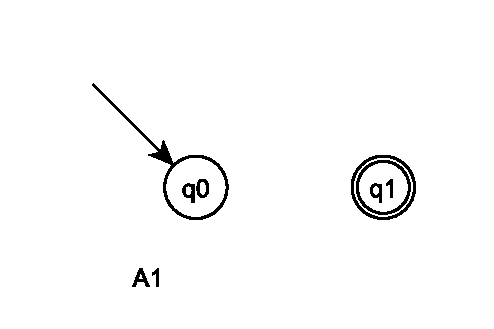
\includegraphics[width=0.4\textwidth]{img/4.pdf}}
\end{figure}
$$
	L(A_1) = 0
$$
\begin{figure}[H]
	\centerline{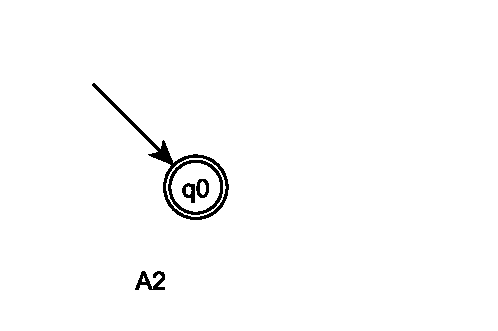
\includegraphics[width=0.4\textwidth]{img/5.pdf}}
\end{figure}
$$
	L(A_2) = \left\{\varepsilon\right\}
$$
\begin{figure}[H]
	\centerline{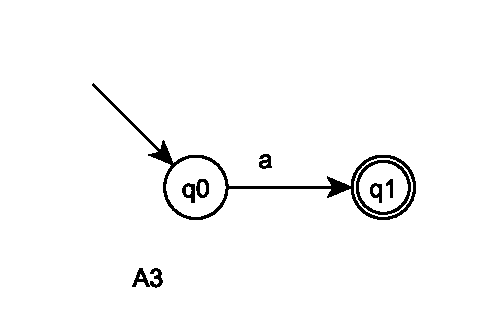
\includegraphics[width=0.4\textwidth]{img/6.pdf}}
\end{figure}
$$
	L(A_3) = \left\{a\right\}, a \in \Sigma
$$
Let $A_1 = (Q_1, \Sigma, \delta_1, q_{01}, F_1)$ and $A = (Q_2, \Sigma, \delta_2, q_{02}, F_2)$ be finite state automata; the language $L(A_1) \cup L(A_2)$ is accepted by a finite state automaton $A_4$:
\begin{figure}[H]
	\centerline{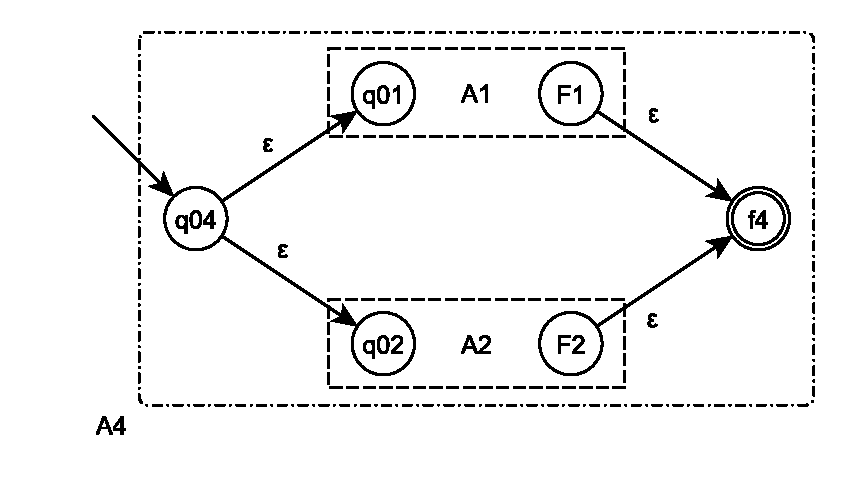
\includegraphics[width=0.7\textwidth]{img/7.pdf}}
\end{figure}

The language $L(A_1)L(A_2)$ is accepted by a finite state automaton $A_5$:
\begin{figure}[H]
	\centerline{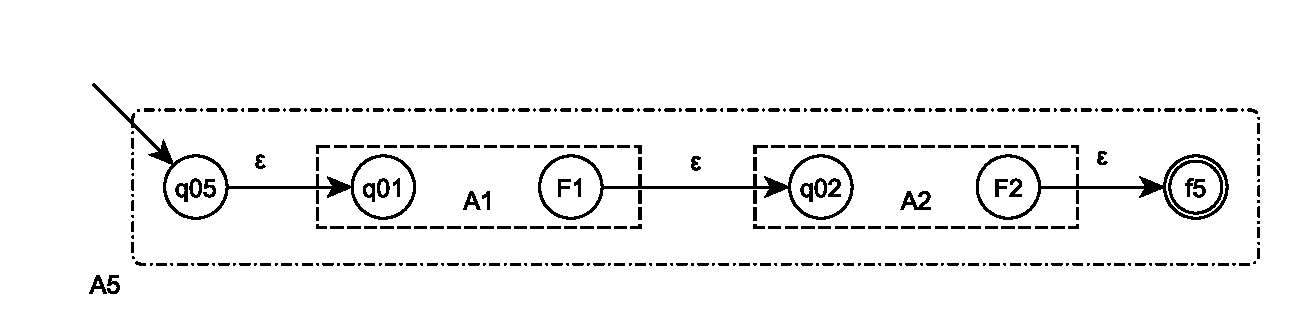
\includegraphics[width=1\textwidth]{img/8.pdf}}
\end{figure}

The language $L(A_1)^\ast$ is accepted by a finite state automaton $A_6$:
\begin{figure}[H]
	\centerline{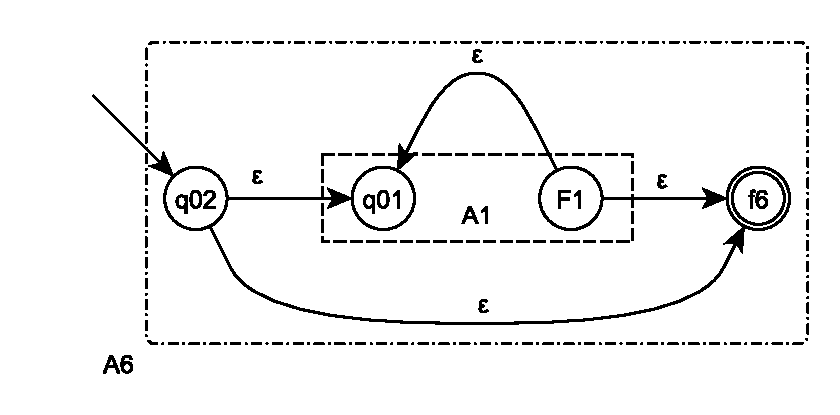
\includegraphics[width=0.7\textwidth]{img/9.pdf}}
\end{figure}

\section{Non-Deterministic Finite State Automata with $\varepsilon\text{-transition}$ ($\varepsilon\text{-NFA}$)}
In the construction of a Finite State Automaton from regular expressions, the $\varepsilon\text{-transitions}$ make the automata \emph{non-deterministic}.
The function $\varepsilon\text{-closure}(q)$ gives the set of states that can be reached (recursively) from state $q$ with empty string.

\subsection{Equivalence of $\varepsilon\text{-NFA}$ and DFA}
Let $N = (Q_n, \Sigma, \delta_n, q_0, F_n)$ be an $\varepsilon\text{-NFA}$; let us construct a DFA $D = (Q_d, \Sigma, \delta_d, \varepsilon\text{-closure}(q_0), F_d)$ where:
\begin{itemize}
	\item $Q_d \subseteq \mathscr{P}(Q_n)$;
	\item $\delta_d(S, a) = \varepsilon\text{-closure}(\cup_i \delta_n(p_i, a))$ where $p_i \in S \in Q_d$;
	\item $F_d \left\{S \middle| S \in Q_d; S \cap F_n \neq \emptyset\right\}$
\end{itemize}
By construction $L(D) = L(N)$.

\section{Finite Automaton $\equiv$ Regular Languages}
\begin{itemize}
	\item Let $G = (N, T, P, S)$ be a \underline{Right-Regular} grammar; let us construct an FA $A = (Q, T, \delta, S, F)$ where:
	\begin{itemize}
		\item $Q = N \cup \left\{\Omega\right\}$ with $\Omega \in N$;
		\item $F = \left\{\Omega\right\}$;
		\item $
			\delta = \begin{Bmatrix}
				\delta(A, a) = B \quad \text{if} \quad A \to aB \in P \\
				\delta(A, a) = \Omega \quad \text{if} \quad A \to a \in P
			\end{Bmatrix}
		$
	\end{itemize}
	By construction $L(G) = L(A)$.
	\item Let $G = (N, T, P, S)$ be a \underline{Left-Regular} grammar; let us construct an FA $A = (Q, T, \delta, I, \left\{S\right\})$ where:
	\begin{itemize}
		\item $Q = N \cup \left\{I\right\} \quad \text{with} \quad I \notin N$;
		\item $F = \left\{S\right\}$;
		\item $
			\delta = \begin{Bmatrix}
				\delta(B, a) = B \quad \text{if} \quad A \to Ba \in P \\
				\delta(I, a) = \Omega \quad \text{if} \quad A \to a \in P
			\end{Bmatrix}
		$
	\end{itemize}
	By construction $L(G) = L(A)$.
\end{itemize}

\section{Minimum-State DFA}
Let $DFA = (Q, \Sigma, \delta, q_0, F)$ be a deterministic finite automaton, then:
\begin{itemize}
	\item two states $p$ and $q$ of DFA are distinguishable if there is a string $w \in \Sigma^\ast$ such that $\delta(p, w) \in F$ and $\delta(q, w) \in F$;
	\item two states $p$ and $q$ of DFA are equivalent ($p \equiv q$) if they are \emph{non-distinguishable} for any string $w \in \Sigma^\ast$.
\end{itemize}
A DFA is \emph{minimum-state} if it does not contain equivalent states.

Two states $p$ and $q$ of a DFA are $m\text{-equivalent}$ ($p \equiv_m q$) if they are non-distinguishable for all strings $w \in \Sigma^\ast$ with $\|w\| \leq m$.
The equivalent states can be determined by partitioning the set $Q$ in classes of $m\text{-equivalent}$ states, for $m = 0, 1, \ldots, \|Q\| - 2$.

\section{Complement of a Regular Language}
The complement of a regular language is a regular language.

Let $DFA = (Q, \Sigma, \delta, q_0, F)$ be a completely specified deterministic finite automaton, that is there is a transition on every symbol of $\Sigma$ from every state.
The automaton $DFA_c = (Q, \Sigma, q_0, Q - F)$ accepts the language
$$
	L(DFA_c) = \Sigma^\ast - L(DFA) = \neg L(DFA)
$$

\section{Intersection of Regular Languages}
The intersection of two regular languages is a regular language.
$$
	L_1 \cap L_2 = \neg (\neg L_1 \cup \neg L_2)
$$
Let $DFA_1 = (Q_1, \Sigma, \delta_1, q_{01}, F_1)$ and $DFA_2 = (Q_2, \Sigma, \delta_2, q_{02}, F_2)$; the automaton $DFA1 = (Q_1 \times Q_2, \Sigma, \delta, (q_{01}, q_{02}), F_1 \times F_2)$ accepts the language
$$
	L(DFA_1) = L(DFA1) \cap L(DFA_2)
$$

\section{Equivalence of Regular Languages}
It is possible to test if two regular languages are the same:
\begin{itemize}
	\item $DFA_1 = (Q_1, \Sigma, \delta_1, q_{01}, F_1)$;
	\item $DFA_2 = (Q_2, \Sigma, \delta_2, q_{02}, F_2)$.
\end{itemize}
Let us find the equivalence states in the set $Q_1 \cup Q_2$:
$$
	\text{if} \quad q_{01} \equiv q_{02} \quad \text{then} \quad L(DFA_1) = L(DFA_2)
$$

\chapter{Context-Free Languages (CFL)}
\section{Parse Trees}
A parse tree for a context-free grammar (CFG) $G = (N, T, P, S)$ is a tree where:
\begin{itemize}
    \item the root is labelled by the start symbol;
    \item each interior node is labelled by a symbol in $N$;
    \item each leaf is labelled by a symbol in $N \cup T \cup \left\{\varepsilon\right\}$;
    \item an interior node labelled by $A$ has a children labelled by $x_1, x_2, \ldots, x_n$ only if $A \to x_1, x_2, \ldots, x_n$ is a production of $P$.
\end{itemize}
Yield of a parse tree is a string obtained by concatenating the labels of the leaves.

\section{Leftmost/Rightmost Derivation}
\subsubsection{Leftmost Derivation}
The leftmost non-terminal symbol is replaced at each derivation step.
\subsubsection{Rightmost Derivation}
The rightmost non-terminal symbol is replaced at each derivation step.

\section{Ambiguity}
Every string in a CFL has at least one parse tree; each parse tree has just one leftmost derivation and just one rightmost derivation.
A context-free grammar is \emph{ambiguous} if there is at least one string in its language having two different parse trees; a CFL is inherently ambiguous if all its grammars are ambiguous.

\section{Eliminating Useless Symbols in a Context-Free Grammar}
A symbol $X$ is useful for a $CFG = (N, T, P, S)$ if there is some derivations $S \Rightarrow^\ast aX\beta \Rightarrow^\ast w \in T^\ast$.
\begin{itemize}
    \item a useful symbol $X$ generates a non-empty languages: $X \Rightarrow^\ast x \in T^\ast$;
    \item a useful symbol $X$ is reachable: $S \Rightarrow^\ast \alpha X\beta$.
\end{itemize}
Eliminating useless symbols from a grammar will not change the generated language:
\begin{enumerate}
    \item eliminate symbols generating an empty language;
    \item eliminate unreachable symbols.
\end{enumerate}
\subsubsection{Finding Symbols Generating Non-Empty Languages}
\begin{itemize}
    \item every symbol of $T$ generates a non-empty language;
    \item if $A \to \alpha$ and all symbols in $\alpha$ generate a non-empty language, then $A$ generates a non-empty language.
\end{itemize}
\subsubsection{Finding Reachable Symbols}
\begin{itemize}
    \item the start symbol $S$ is reachable;
    \item if $A \to \alpha$ and $A$ is reachable, all symbols in $\alpha$ are reachable.
\end{itemize}

\section{$\varepsilon\text{-productions}$ in CFG}
According to the Chomsky classification, only \emph{Type 0 grammars} can have $\varepsilon\text{-productions}$; anyway the languages generated by CFGs that contain $\varepsilon\text{-productions}$ are CFL.

A context-free grammar $G_1$ with $\varepsilon\text{-productions}$ can be transformed into an equivalent CFG $G_2$ without $\varepsilon\text{-productions}$:
$$
    L(G_2) = L(G_1) - \left\{\varepsilon\right\}
$$
If $A \to x_1, \ldots, x_i, \ldots, x_n$ is in $P_1$ and $x_i \Rightarrow^\ast \varepsilon$, then $P_2$ will contain $A \to x_1 \ldots x_i \ldots x_n$ and $A \to x_1 \ldots x_{i - 1} x_{i + 1} \ldots x_n$.

\section{Pushdown Automata (PDA)}
A PDA is a 7-tuple $P = (Q, \Sigma, \Gamma, \delta, q_0, Z_0, F)$ where:
\begin{description}
    \item[$Q:$] finite (non-empty) set of states;
    \item[$\Sigma:$] alphabet of input symbols;
    \item[$\Gamma:$] alphabet of stack symbols;
    \item[$\delta:$] transition function
    $$
        \delta: Q \times (\Sigma \cup \left\{\varepsilon\right\}) \times \Gamma \to \left\{(p, \gamma) \middle| p \in Q; \gamma \in \Gamma^\ast \right\}
    $$
    \item[$q_0:$] start state ($q_0 \in Q$);
    \item[$Z_0:$] start stack symbol ($Z_0 \in \Gamma$);
    \item[$F:$] set of final states ($F \subseteq Q$).
\end{description}

\subsection{Transitions of a PDA}
\begin{itemize}
    \item $\delta(q,a,x) = \left\{(p_1, \gamma_1), \ldots, (p_m, \gamma_m)\right\}$
    From state $q$, with $a$ in input and $x$ on top of the stack:
    \begin{enumerate}
        \item consumes $a$ from the input string;
        \item goes to a state $p_i$ and replace $x$ with $\gamma_i$ (the first symbol of $\gamma_i$ goes on top of the stack).
    \end{enumerate}
    \item $\delta(q,\varepsilon,x) = \left\{(p_1, \gamma_1), \ldots, (p_m, \gamma_m)\right\}$
    From state $q$, with $x$ on top of the stack:
    \begin{enumerate}
        \item no input symbol is consumed;
        \item goes to a state $p_i$ and replaces $x$ with $\gamma_i$ (the first symbol of the stack).
    \end{enumerate}
\end{itemize}

\subsection{Languages Accepted by a PDA}
Language accepted by final state by PDA:
$$
    P = (Q, \Sigma, \Gamma, \delta, q_0, Z_0, F)
$$
$$
    L(P) = \left\{w \middle| w \in \Sigma^\ast; (q_0, w, Z_0) \to^\ast (q, \varepsilon, \alpha); q \in F \right\}
$$
Language accepted by empty stack by the PDA:
$$
    P = (Q, \Sigma, \Gamma, \delta, q_0, Z_0, \emptyset)
$$
$$
    N(P) = \left\{w \middle| w \in \Sigma^\ast; (q_0, w, Z_0) \to^\ast (q, \varepsilon, \varepsilon) \right\}
$$

\subsection{PDA Languages $\equiv$ Context-Free Languages}
Let $G = (N, T, P, S)$ be a context-free grammar; let us construct a $PDA = (\left\{q\right\}, T, \Gamma, \delta, q, S, \emptyset)$ where:
\begin{itemize}
    \item $\Gamma = N \cup T$;
    \item $\delta = \begin{Bmatrix}
        \delta(q, \varepsilon, A) = \left\{(q, \alpha) \quad \text{for each} \quad A \to \alpha \in P \right\} \\
        \delta(q, a, a) = \left\{(q, \varepsilon) \quad \text{for each} \quad a \in T \right\}
        \end{Bmatrix}$
\end{itemize}
PDA accepts $L(G)$ by empty stack, making a sequence of transitions corresponding to a leftmost derivation.

\chapter{Turing Machines (TM)}

\part{Compilers}

\chapter{Compiler Structure (CS)}
\section{Compiler Structure}
\begin{figure}[H]
    \centerline{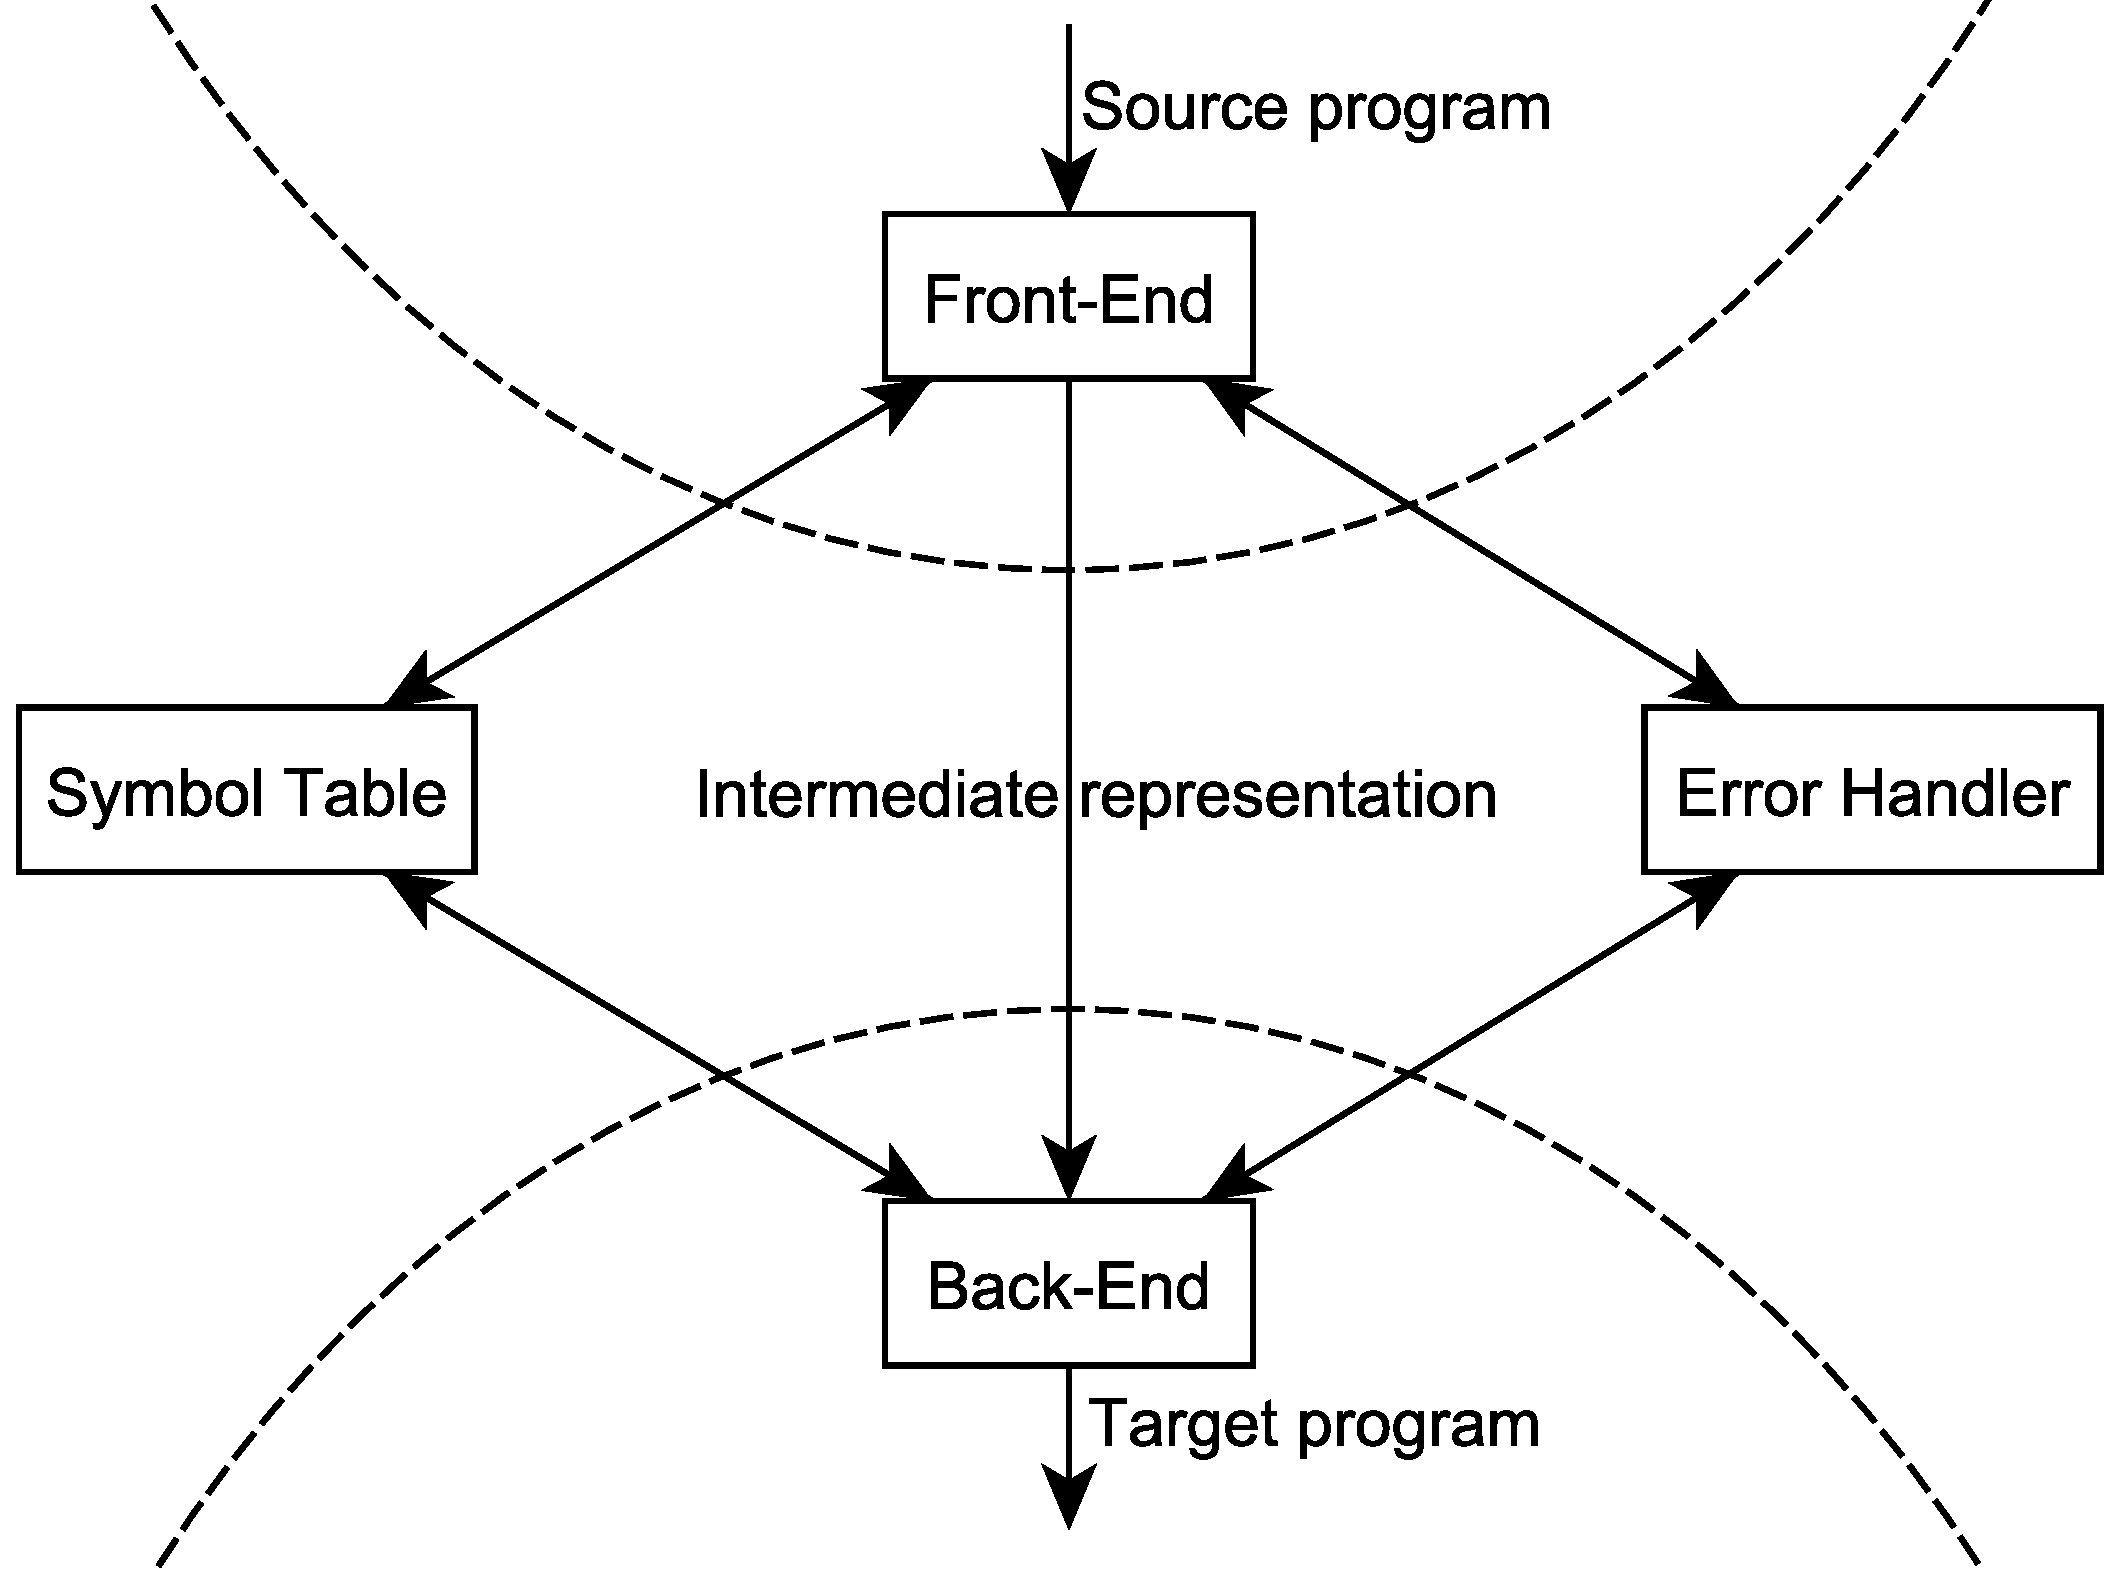
\includegraphics[width=0.7\textwidth]{img/10.pdf}}
\end{figure}

\subsection{Front-End}
\begin{figure}[H]
    \centerline{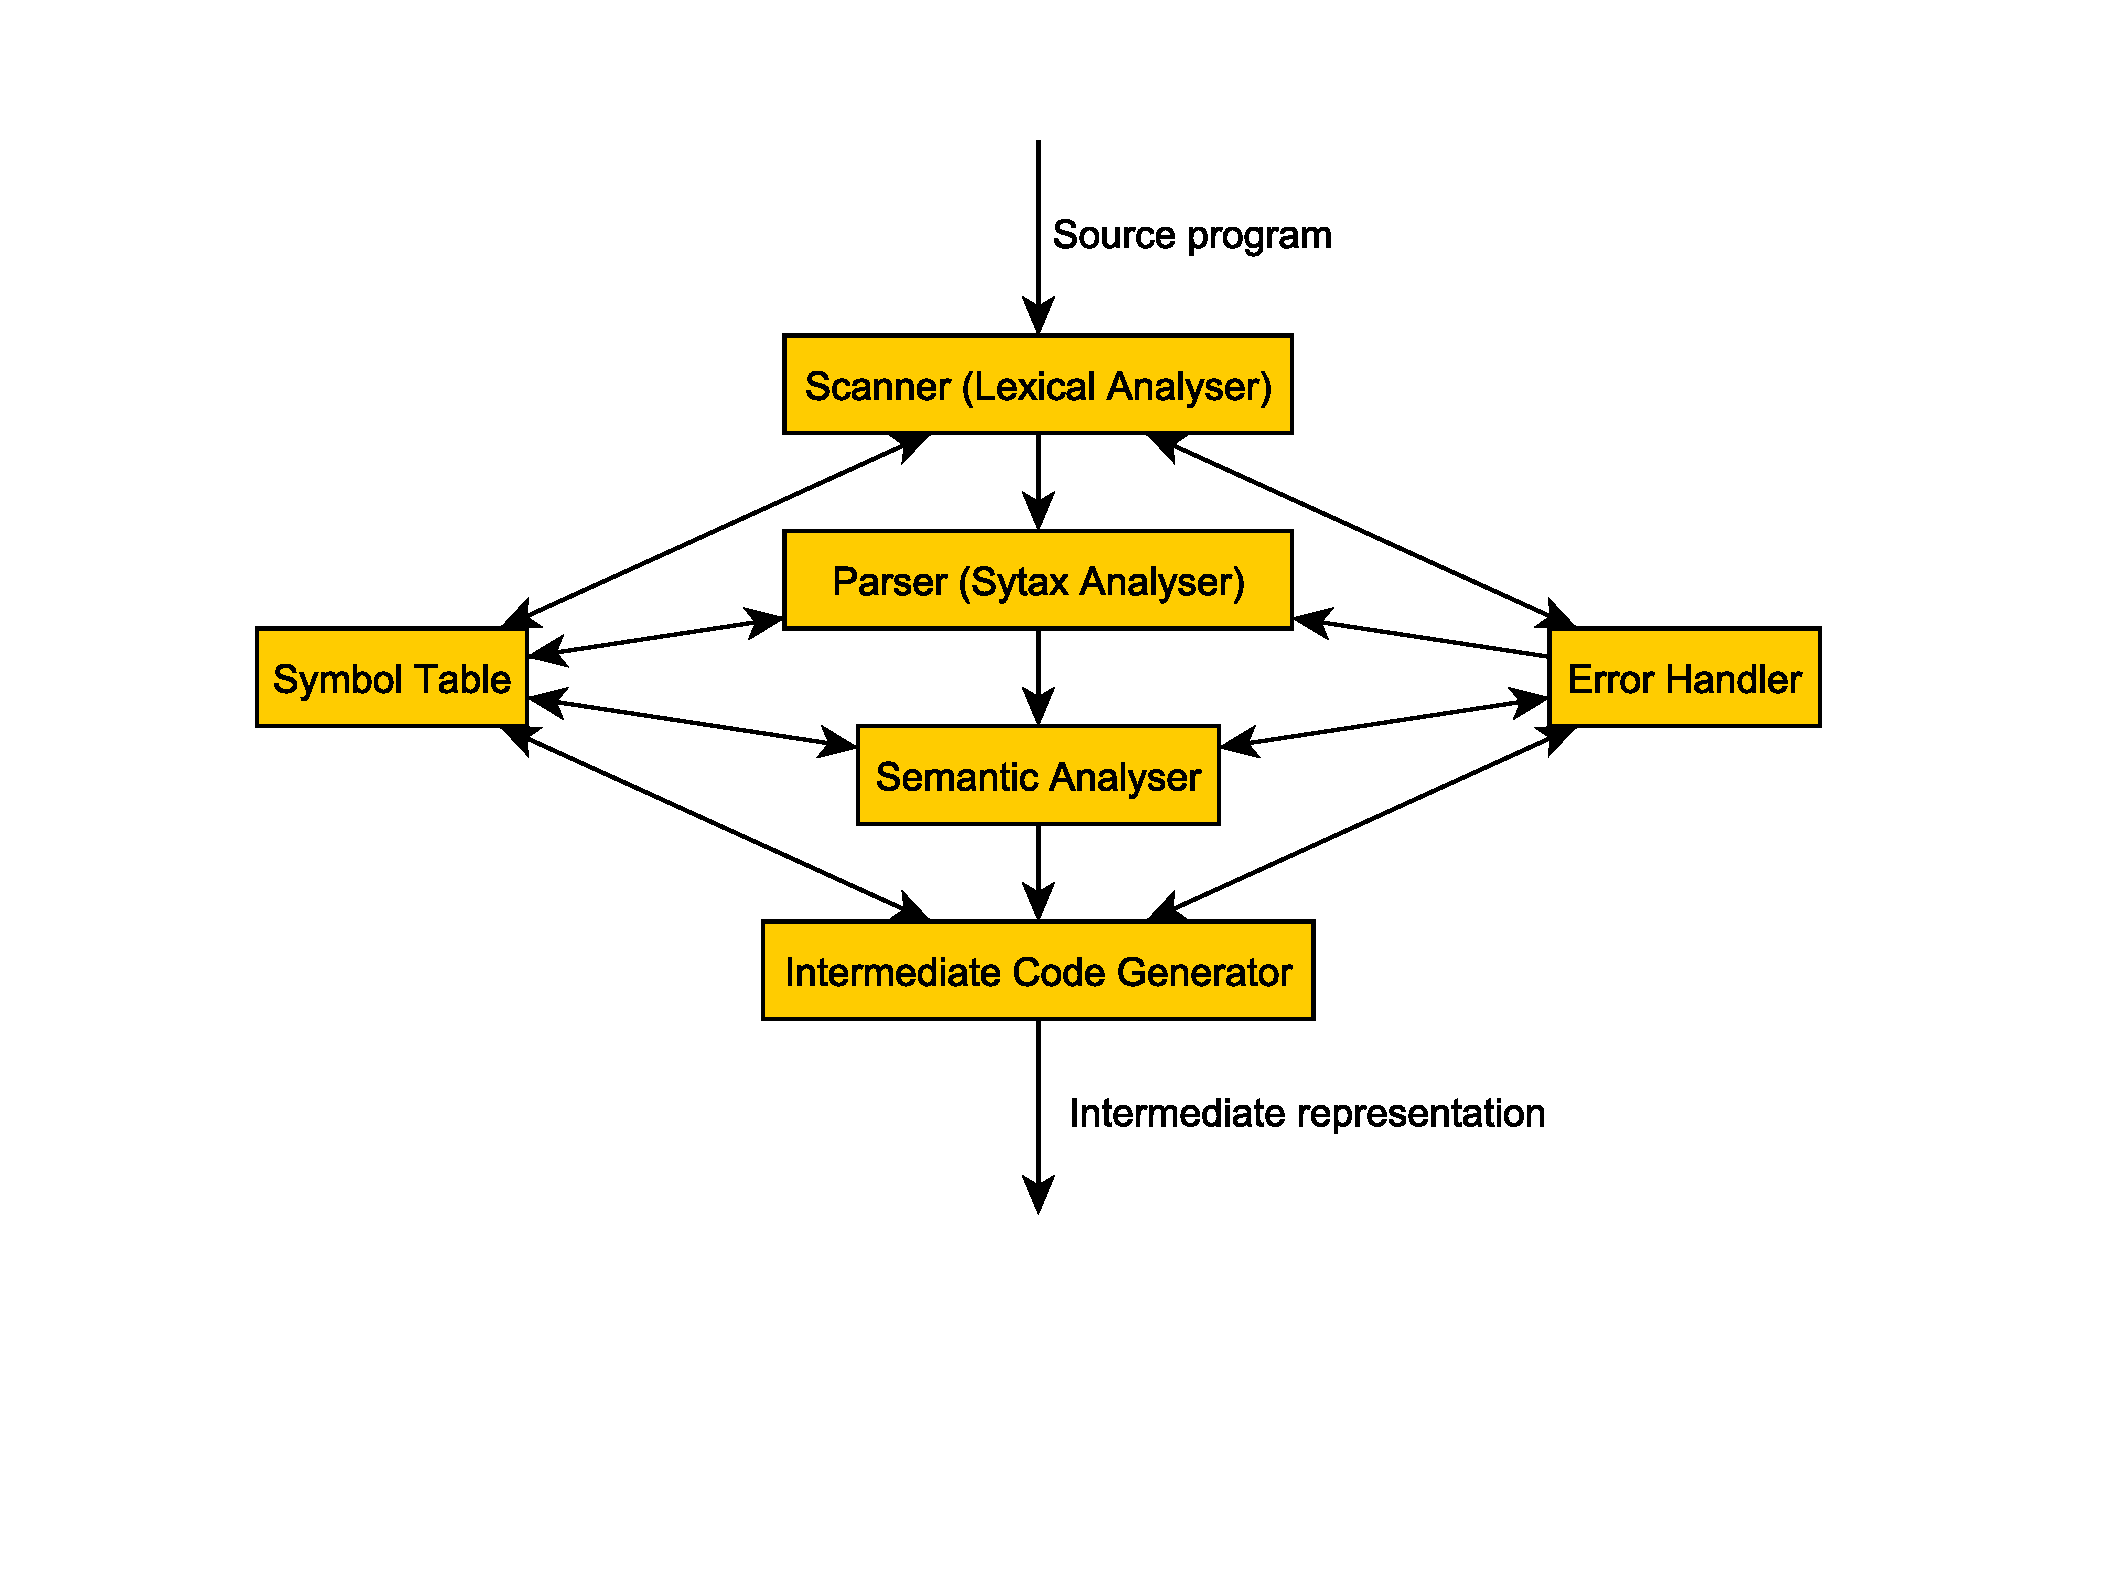
\includegraphics[width=0.8\textwidth]{img/11.pdf}}
\end{figure}

\subsection{Back-End}
\begin{figure}[H]
    \centerline{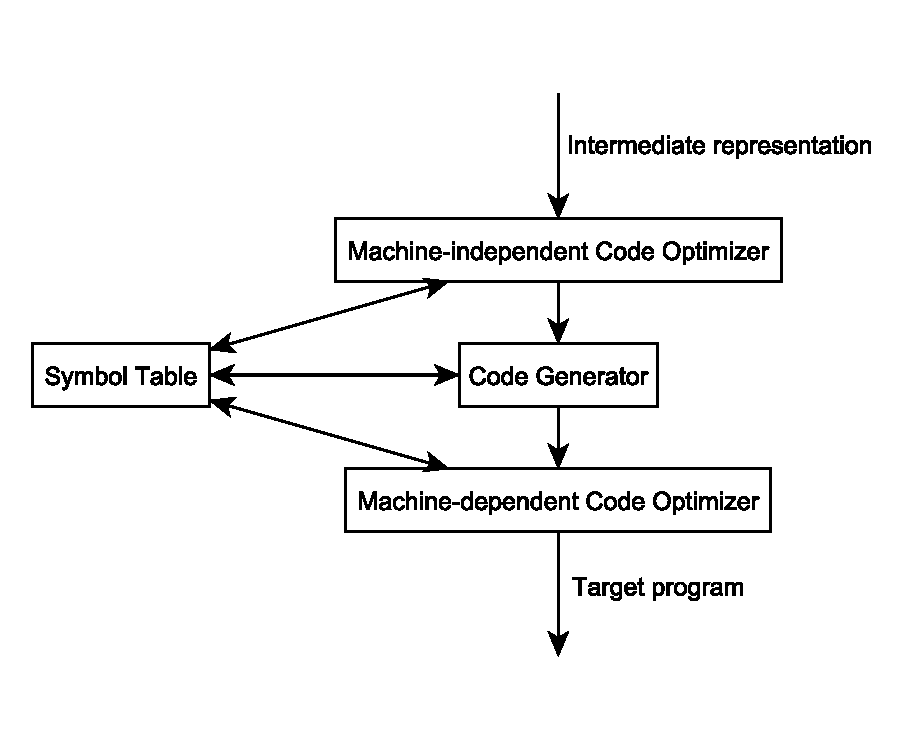
\includegraphics[width=0.8\textwidth]{img/12.pdf}}
\end{figure}

\chapter{Lexical Analysis (LA)}
\begin{figure}[H]
	\centerline{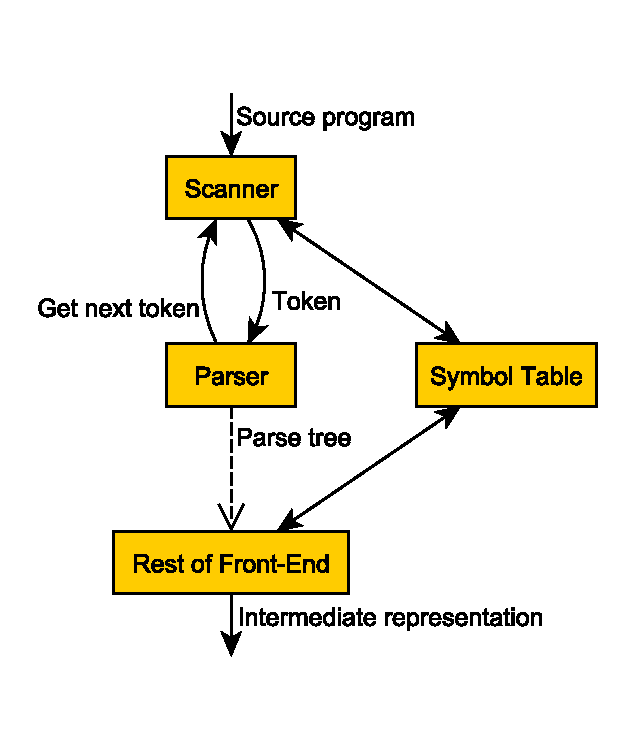
\includegraphics[width=0.6\textwidth]{img/13.pdf}}
\end{figure}

Tokens are terminal symbols in the grammar for the source language.
Lexeme is a string of characters in the source program treated as a lexical unit.
Pattern is a representation of the set of lexemes associated with a token.

\section{Role of a Scanner}
Upon receiving a ``get next token'' command from the parser, the scanner reads input characters until it can identify a token.
Scanner simplifies the job of the parser:
\begin{itemize}
	\item it discards as many irrelevant details as possible;
	\item parser rules are only concerned with tokens, not with lexemes.
\end{itemize}
Also, scanner improves compiler efficiency.

\section{Regular Definitions}
A regular definition is a sequence of definitions:
$$
	d_1 \to r_1; d_2 \to r_2; \ldots; d_n \to r_n
$$
Each $d_i$ is a distinct name (token); each $r_i$ is a regular expression, over $\Sigma \cup \left\{d_1, \ldots, d_{i-1}\right\}$ representing a pattern.

The task of constructing a lexical-analyser is simple enough to be automated.
A lexical-analyser generator transforms the specification of a scanner into a program implementing a finite automaton accepting the specified lexemes.

\chapter{Syntax Analysis (SA)}
\section{Role of a Parser}
The parser obtains a string of tokens from the scanner and:
\begin{itemize}
	\item verifies that the string can be generated by the grammar for the source language, trying to build a parse tree;
	\item reports syntax errors and continues processing the input.
\end{itemize}
There are two different types of parser:
\begin{itemize}
	\item \emph{Bottom-Up} parsers build parse trees from the bottom (leaves) to the top (root);
	\item \emph{Top-Down} parsers build parse trees from the top (root) to the bottom (leaves).
\end{itemize}

\section{Bottom-Up Parsing}
Bottom-Up parsing attempts to construct a parse tree for an input string beginning at the leaves (the bottom).
this construction process reduces an input string to the start symbol of a grammar; at each reduction step the right side of a production is replaced by its left side symbol, tracing out a rightmost derivation in reverse.

\section{Handles}
If a string $\alpha \beta w$ can be produced by a rightmost derivation $S \Rightarrow^\ast_{RM} \alpha AW \Rightarrow^\ast_{RM} \alpha \beta w$, then $A \to \beta$ is an handle of $\alpha \beta w$ ($w \in T^\ast$ because $A \to \beta$ is the last applied rule).

\section{Actions of a Shift-Reduce Parser}
\begin{description}
	\item[Shift]\mbox{}\\
	the next input symbol is shifted onto the top of the stack;
	\item[Reduce]\mbox{}\\
	the left end of the handle must be located within the stack; it must be decided with what non-terminal to replace the handle;
	\item[Accept]\mbox{}\\
	parsing is successfully completed;
	\item[Error]\mbox{}\\
	a syntax error has occurred.
\end{description}
A strategy for making parsing decision is needed in order to avoiding conflicts with decision between shift and reduce operations.

\section{LR Parser}
LR parsers are a type of bottom-up parsers that handle deterministic context-free languages in guaranteed linear time.
The \emph{LALR} parsers and the \emph{SLP} parsers are common variants of LR parsers.
LR parsers are of ten generated from a formal grammar for the language by a parser generator tool.

The name LR is an acronym: the \emph{L} means that the parser reads input text in one direction without baking up; that direction is typically ``left-to-right'' within each line, and ``top-to-bottom'' across the lines of the full input file.
The \emph{R} means that the parser produces a reversed rightmost derivation; it does a bottom-up parse.

The name LR is often followed by a numeric qualifier, as in $LR(1)$ or sometimes $LR(k)$.
To avoid backtracking or guessing, the LR parser is allowed to peek ahead a $k$ lookahead input symbols before deciding how to parse earlier symbols.

\subsection{$LR(0)$ Items}
An $LR(0)$ item of a CFG grammar $G$ is a production of $G$ with a dot at some position of the right side; an item indicate how much of a production we have seen at a given point in the parsing process.
The dot indicates the current position of the parser and an item with the dot at the end is called \emph{complete} (that is all the right side of the production has been recognized).

\subsection{Viable Prefixes}
A viable prefix of a string $\gamma$ is a prefix that can appear on the stack of a shift reduce parser.

To recognize viable prefixes:
\begin{itemize}
	\item the sets of viable prefixes are regular languages;
	\item the FA that recognizes them can guide a parser in making decisions;
	\item the valid $LR(0)$ items of a CFG grammar are the states of an NFA recognizing viable prefixes;
	\item a DFA equivalent to such NFA will have states corresponding to sets of $LR(0)$ items and transitions labelled by symbols in viable prefixes.
\end{itemize}

The function $closure(I)$ finds the set of $LR(0)$ items that recognizes the same viable prefix.
The function $goto(I, x)$ finds the set of $LR(0)$ items that is reached from the set $I$ with symbol $x$.

Given a CFG grammar $G = (N, T, P, S)$, the function $items(G)$ constructs the collection $C = \left\{I_0, I_1, \ldots, I_m\right\}$ of DFA states.

The function $lr_0table(G)$ constructs the $LR(0)$ parsing table for the CFG $G$.
The initial state of the parser is the one constructed from the set of items containing $S' \to \bullet S$.

\subsection{Conflicts in Parsing Tables}
Parsing table entries defined in multiple ways determines parsing action conflicts:
\begin{description}
	\item[Shift/Reduce]\mbox{}\\
	some entry in the action table contains both a shift and reduce action;
	\item[Reduce/Reduce]\mbox{}\\
	some entry in the action table contains more reduce actions.
\end{description}

\subsection{$LR(0)$ Grammars}
A grammar $G$ is $LR(0)$ if the action table generated by the function $lr_0table(G)$ does not comprise conflicts.
$LR(0)$ grammars are ``non-ambiguous''.

\subsection{$LR(0)$ Parsers}
An $LR(0)$ parser:
\begin{itemize}
	\item scans the input from left to right;
	\item constructs a rightmost derivation in reverse;
	\item uses zero lookahead input symbols in making parsing decision.
\end{itemize}
The class of languages that can be parsed using $LR(0)$ parsers is a proper subset of the deterministic CFL.

\subsection{$LR(k)$ Parsers}
More powerful parsers can be constructed when more than zero lookahead input symbols are used in making parsing decision.

\subsection{First and Follow Sets}
With respect to a CFG, given a non-terminal symbol $x$ and a string $\gamma$ of terminal and non-terminal symbols:
\begin{description}
	\item[$nullable(x):$] is true if $x$ can derive an empty string;
	\item[$nullable(\gamma):$] is true if each symbol in $\gamma$ is nullable;
	\item[$first(\gamma):$] is the set of terminals that can begin strings derived from $\gamma$;
	\item[$follow(\gamma):$] is the set of terminals that can immediately follow $x$.
\end{description}

\subsection{Simple LR Parsing Table}
The function $slrTable(G)$ constructs the SLR parsing table from the CFG $G$.

\subsection{$LR(k)$ parsers (bis)}
$Follow(A)$ is the set of terminals that can immediately follow A in any string generated by a given grammar $G$.
It takes into account all the contexts where A can appear; by taking into account the specific context of $A$ when the rule $A \to \alpha$ is applied, it could be possible to set $A$ \underline{reduce} $A \to \alpha$ action for a subset of $follow(A)$, thus avoiding further potential conflicts.

\subsection{$LR(1)$ Items}
An $LR(1)$ item of a context free grammar $G$ is a production of $G$ with a dot at some position of the right side and a lookahead (terminal of $\$$) symbol.

An $LR(1)$ item $[A \to \alpha; a]$ calls for a reduction by $A \to \alpha$ only if the next input symbol is $a$ ($follow(A) = a$).

We say item $[A \to \beta_1 \bullet \beta_2, a]$ is valid for a viable prefix $\alpha\beta_1$ if:
\begin{itemize}
	\item there is a derivation $S \Rightarrow^\ast_{RM} aAw \Rightarrow^\ast_{RM} \alpha\beta_1\beta_2w$;
	\item either $a$ is the first symbol of $w$, or $w$ is $\varepsilon$ and $a$ is $\$$.
\end{itemize}
The valid $LR(1)$ items of a CFG are the states on an NFA recognizing viable prefixes.
A DFA equivalent to such NFA will have states corresponding to sets of $LR(1)$ items and transitions labelled by the symbols of the viable prefixes.

The function $closure_1(I)$ finds the set of $LR(1)$ items that recognize the same viable prefix; the function $goto_1(I, x)$ finds the set of $LR(1)$ items that is reached from the set $I$ with symbol $x$.
Given a CFG $G = (N, T, P, S)$, the function $items_1(G)$ constructs the collection $C = \left\{I_0, I_1, \ldots, I_n\right\}$ of DFA states.
The function $lr_1table(G)$ constructs the $LR(1)$ parsing table for the CFG $G$.

\subsection{$LR(1)$ Parsers}
An $LR(1)$ parser:
\begin{itemize}
	\item scans the input from left to right;
	\item constructs a rightmost derivation in reverse;
	\item uses one lookahead input symbol in making parsing.
\end{itemize}
The class of languages that can be parsed using $LR(1)$ parsers is exactly the class of deterministic CFL.

\subsection{Lookahead $LR(1)$ parsers (LALR)}
$LR(1)$ parsing tables can be very large (several thousand states) for grammars generating common programming languages; SLR parsing tables for the same languages are much smaller, but can contain \underline{conflicts}.
$LALR(1)$ parsing tables have the same states of SLR tables and can conveniently express more programming languages.

\subsection{$LALR(1)$ Parsing Tables}
Two sets of $LR(1)$ items have the same core if they are identical except for the lookahead symbols.
A set of $LALR(1)$ items is the union of sets of $LR(1)$ items having the same core.

The merging of states with common cores can never produce a ``shift/reduce'' conflict which was not present in one of the original states (shift actions depend only on the core, not the lookahead); anyway some ``reduce/reduce'' conflicts can occur after merging.

The class of languages that can be parsed using $LALR(1)$ parsers is a proper subset of the deterministic CFL.

\subsection{Using Ambiguous Grammars}
Ambiguous grammars are not $LR(k)$.
Some ambiguous grammars provide shorter and more natural specifications that any equivalent unambiguous grammar.
In some cases disambiguating rules, such as precedence and associativity, can be specified; the resulting parser can be more efficient.
Ambiguous constructs should be used sparingly and in a strictly controlled fashion.

\subsection{Error Recovery in LR Parsing}
Blanks in LR parsing tables mean error actions and cause the parser to stop.
This behaviour would be unkind to the user, who would like to have all the errors reported, not just the first one.
Local error recovery mechanism use a special error symbol to allow parsing to resume; whenever the error symbol appears in a grammar rule, it can match a sequence of erroneous input symbols.

\subsection{Recovery Using the Error Symbol}
Let $A \to error \quad \alpha$ be a grammar production; in the construction of the parsing table:
\begin{itemize}
	\item $error$ is considered a terminal symbol;
	\item error productions are treated as ordinary production.
\end{itemize}
On encountering an error action (a blank in the table), the parser:
\begin{enumerate}
	\item pops the stack until a state is reached where the action for error is shift (a state including an item $A \to \bullet error \quad \alpha$);
	\item shifts a fictitious $error$ token out the stack, as though $error$ was found on input;
	\item skips ahead on the input discarding symbols until a substring is found that can be reduced to $\alpha$;
	\item reduces the handle $error \quad \alpha$ (at this point on top of the stack) to $A$.;
	\item emits a diagnostic message;
	\item resumes normal parsing.
\end{enumerate}
Error rules may introduce both ``shift/reduce'' and ``reduce/reduce'' conflicts; they cannot be inserted anywhere into an LALR grammar,.
This error recovery mechanism is not powerful enough to correctly report all syntactic errors.

\subsection{LR Parser Generators}
An LR parser generator transforms the specification of a parser into a program implementing an LR parser.
CUP produces Java programs implementing $LALR(1)$ parsers.

\section{Top-Down Parsing}
Top-down parsing attempts to construct a parse tree for an input string starting at the root and working down towards the levaes.
This construction process creates the nodes of the tree in pre-order until it obtains the input string.
At each creation step the left side symbol of a production is replaced by its right side, tracing out a leftmost derivation.

\section{Left-Recursive Grammars}
A production like $A \to A\alpha$ is called ``left-recursive production''; a grammar is left-recursive if it can generate a derivation $A \Rightarrow^\ast A\alpha$.
A left-recursive grammar can cause a top-down parser to go into an infinite loop.
Left-recursive productions can be replaced by right-recursive productions:
%% the following math section generates some problems but the output is good...
$$
\text{problem here with math environment}
%	\[
%		A \to A\alpha | \beta \equiv \left\{
%		\begin{array}{c}
%			A \to \beta R \\
%			R \to \alpha R
%		\end{array}
%		\right.
%	\]
$$
($\beta$ doesn't start with $A$)
$$
	A \Rightarrow^\ast \beta\alpha^\ast
$$

\section{Predictive Parsing}
Backtracking can be avoided if it is possible to detect alternative rule among $A \to \alpha_1 | \alpha_2 | \ldots | \alpha_n$ has to be applied, by considering the current input symbol.

\section{$LL(1) Grammars$}
A grammar $G$ is $LL(1)$ if its predictive parsing table has no multiply-defined entries.
No ambiguous or left-recursive grammar can be $LL(1)$.

An $LL(1)$ parser:
\begin{itemize}
	\item scans the input from left to right;
	\item constructs a leftmost derivation;
	\item uses one lookahead input symbol in making parsing decision.
\end{itemize}

The class of languages that can be parsed using $LL(1)$ parser is a proper subset of the deterministic CFL parser into a program implementing an LL parser.

\chapter{Syntax-Directed Translation (SDT)}
\section{Syntax-Directed Definitions}
A Syntax-Directed Definition (SDD) is a context-free grammar in which:
\begin{itemize}
	\item each symbol can have an associated set of attributes (numbers, types, table references, strings, memory locations, \ldots);
	\item each production can have an associated set of semantic rules (evaluating attributes, interacting with the symbol table, writing lines of intermediate code to a buffer, printing messages, \ldots).
\end{itemize}

\subsection{Inherited and Synthesized Attributes}
A semantic rule associated with a production $A \to XYZ$ can refer only attributes associated with symbols in that production:
\begin{description}
	\item[Inherited Attributes] are evaluated in rules where the associated symbol is on the right side of the production;
	\item[Synthesized Attributes] are evaluated in rules where the associated symbol is on the left side of the production.
\end{description}

\begin{table}[h]
	\centering
	\begin{tabular}{l|l}
		Productions & Semantic Rules \\ \hline
		$L \to Em$ & $print(E.val)$ \\ \hline
		$E \to E_1 + T$ & $E.val = E_1.val + T.val$ \\ \hline
		$E \to T$ & $E.val = T.val$ \\ \hline
		$T \to T_1 \ast F$ & $T.val = T1_.val \ast F.val$ \\ \hline
		$F \to digit$ & $F.val = digit.lexval$
	\end{tabular}
	\caption{SDD example for a desk calculator.}
\end{table}
Each of the non-terminal $E, T, F$ has a single synthesized attribute, named ``val''; the terminal digit has an attribute ``lexval'' which is the integer value returned by the scanner.

\begin{table}[h]
	\centering
	\begin{tabular}{l|l}
		Productions & Semantic Rules \\ \hline
		$D \to TL$ & $L.inh = T.type$ \\ \hline
		$T \to int$ & $T.type = integer$ \\ \hline
		$T \to float$ & $T.type = real$ \\ \hline
		$L \to L_1, id$ & $L_1.inh = L.inh; addtype(L.inh, id.entry)$ \\ \hline
		$L \to id$ & $addtype(L.inh, id.entry)$
	\end{tabular}
	\caption{SDD example for simple declarations.}
\end{table}

\begin{itemize}
	\item the non-terminal $T$ has a synthesized attribute named $type$;
	\item the non-terminal $L$ has a inherited attribute, named $int$;
	\item the terminal $id$ has an attribute entry which is the value returned by the scanner (it points to the symbol table entry for the identifier associated with $id$);
	\item the function $addtype(L.inh, id.entry)$ installs the type $L.inh$ at the symbol table position $id.entry$.
\end{itemize}

\subsection{Evaluation Orders for Syntax Directed Definitions}
An attributes at a node in an annotated parse tree cannot be evaluated before the evaluation of all attributes upon which its value depends.
The dependency relations in a parse tree define a dependency graph representing the flow of information among attributes and semantic rules.
Any topological sort of the dependency graph is an allowable order of evaluation for an SDD.
Any directed acyclic graph has at least one topological sort.

\subsection{Ordering the Evaluation of SDD}
Syntax-directed translation can be performed by:
\begin{itemize}
	\item creating a parse tree;
	\item visiting the parse tree an evaluating an SDD according to a topological sort of the dependency graph.
\end{itemize}
It is extremely complex to tell whether, for a given SDD, there are any parse trees whose dependency graphs have cycles.
It is possible to define classes of DSS (S-attribtues and L-attributes) in ways that:
\begin{itemize}
	\item cycles are not allowed;
	\item translation is performed in connection with top-down or bottom-up parsing, without explicitly creating the tree nodes.
\end{itemize}

\subsection{S-Attributes Definitions}
An SDD is S-attributed if every attribute is synthesized.
All semantic rules use only attributes of symbols in the right side of the associated productions.

\begin{table}[h]
	\centering
	\begin{tabular}{l|l}
		Productions & Semantic Rules \\ \hline
		$L \to En$ & $print(E.val)$ \\ \hline
		$E \to E_1 + T$ & $E.val = E_1.val + T.val$ \\ \hline
		$E \to T$ & $E.val = T.val$ \\ \hline
		$T \to T_1 \ast F$ & $T.val = T_1.val \ast F.val$ \\ \hline
		$T \to F$ & $T.val = F.val$ \\ \hline
		$F \to (E)$ & $F.val = E.val$ \\ \hline
		$F \to digit$ & $F.val = digit.lexval$ 
	\end{tabular}
\end{table}

\begin{figure}[H]
	\centerline{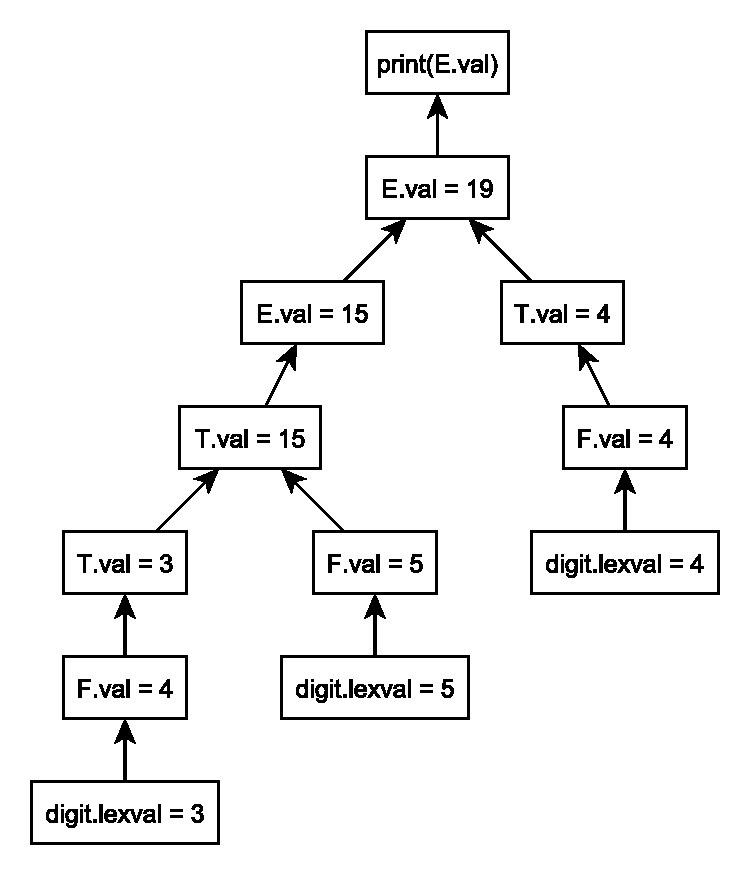
\includegraphics[width=0.6\textwidth]{img/14.pdf}}
	\caption{Dependency trees of S-attributed definitions}
\end{figure}

\subsection{Evaluation Order for S-Attributed Definitions}
S-Attributed definitions can be evaluated in any bottom-up order.
The evaluation order of function post-order (rootNode) corresponds to the order in which a bottom-up parser creates nodes in a parse tree.

\section{Syntax-Directed Translation Schemes (SDT)}


%\chapter{Semantic Analysis and Intermediate-Code Generation (SA/ICG)}
\chapter{Semantic Analysis (SA)}

\section{Type Expressions}

\chapter{Intermediate-Code Generation (ICG)}
\section{Intermediate Representations}

\section{Scope of Declaration}

\section{Symbol Tables}

\section{Storage Layout for Sequence of Declarations}

\section{Storage for Records}

\section{Translation of Assignment Statements}

\section{Translation of Boolean Expression}

\section{Back-Patching}

\part{Laboratories}
\chapter{Regular Expressions and JFlex Scanner}
\section{Languages}
\begin{description}
    \item[Lexicon] $\to$ scanner JFlex: lexical analyser;
    \item[Syntax] $\to$ parser CUP: syntax and semantic analyser;
    \item[Semantic] $\to$ understanding the meaning of expressions.
\end{description}

\section{JFlex: a Lexical Analysers Generator}
Transforming regular expressions in deterministic finite state automata and implementing them is a long and mechanical process; hence, a lexical analyser (or scanner) automatic generator is often used.

JFlex is a generator which takes as input a set of regular expressions and associated actions, and produces as output a Java program that matches a given input against them.

\subsection{Regular Expressions in JFlex}
\begin{itemize}
    \item Regular expressions describe sequences of ASCII characters using a set of operators;
    \item letters and numbers in the input string are described by the characters themselves;
    \item non-alphabetical characters must be written in quotation marks, to avoid ambiguities with operators;
    \item non-alphabetical characters can be also preceded by the \code{\\};
    \item character classes are identified by square brackets \code{[]}, in which the \code{-} character is used to describe a range of characters:
    \begin{itemize}
        \item \code{[0-9]} $\to$ digit between 0 and 9,
        \item \code{[a-z]} $\to$ lower case letter,
        \item \code{[a-zA-Z0-9]} $\to$ both lower and upper case letter and number;
    \end{itemize}
    \item to include the character \code{-} in a character class, it must be either the first or the last character within the brackets;
    \item the character \code{^} at the beginning of a character class identifies a ``negated character class'' (example: \code{[^0-9]} $\to$ any character except digits);
    \item the symbol \code{.} (dot) identifies any character except newline;
    \item the newline character is described by the following regular expression: \code{\\n\|\\r\|\\r\\n} (note: \code{\\n\|\\r\|\\r\\n} $\to$ one newline only, \code{[\\n\\r]+} $\to$ one or more newlines);
    \item the symbol \code{\\t} identifies the tabulation character;
    \item the operator \code{?} indicates that the preceding expression is optional;
    \item the operator \code{*} indicates that the preceding expression can be repeated 0 or more times;
    \item the operator \code{+} indicates that the preceding expression can be repeated 1 or more times;
    \item the operator \code{\{n\}} represents $n$ repetitions of the precedent regular expression (example: \code{ab\{3\}c} $\to abbbc$);
    \item the operator \code{\{n, m\}} represents a repetition of the regular expression between a minimum of $n$ and a maximum of $m$ (example: \code{ab\{2,4\}c} $\to abbc$, $abbbc$, or $abbbbc$);
    \item the operator \code{\|} represents two alternative expressions (example: \code{ab\|bc} $\to ab$ or $bc$);
    \item parentheses are used to express/modify operators priority, some examples:
    \begin{itemize}
        \item unsigned integers: \code{[0-9]+}
        \item unsigned integers without leading zeros: \code{[1-9][0-9]*}
        \item signed integers: \code{("+"\|"-")?[0-9]+}
        \item floating point number: \code{("+"\|"-")?([1-9][0-9]*"."[0-9]*)\|("."[0-9]+)\|(0"."[0-9]*)}
    \end{itemize}
\end{itemize}

\subsection{Structure of a JFlex Source File}
A JFlex source file has three distinct sections separated by \code{\%\%}:
\begin{itemize}
    \item the first section is called \underline{Code Section}, it contains the user code and can be empty;
    \item the second section is the \underline{Declaration Section} and contains option and declarations;
    \item the third section is called \underline{Rules Section} and contains the lexical rules in the form of \code{regular expression - action} pairs.
\end{itemize}
\begin{lstlisting}[frame=single]
code section
%%
declarations section
%%
rules section
\end{lstlisting}

\subsubsection{Code Section}
All the code lines present in this section are copied without any modification in the generated scanner.
Usually, import statement for Java libraries that will be used in the next sections are inserted here.
Examples:
\begin{lstlisting}
import java.io.*;
import java_cup.runtime.*;
\end{lstlisting}

\subsubsection{Declaration Section}
To simplify the usage of complex or repetitive regular expressions, it is possible to define identifiers for sub-expressions.
Example: \code{integer = [+-]?[1-9][0-9]*}

The sub-expression can be then used in the rules section, writing its name between braces.
Example: \code{\{integer\} \{System.out.print("integer found");\}}

Java code can be included in the declarations section by writing it between \code{\%\{} and \code{\%\}}

\subsubsection{Rules Section}
IN JFlex, each regular expression is associated to an action, which is executed when the input matches the regular expression.
Actions are constituted by snippets of Java code, written between braces.
The simplest action consists in ignoring the matched string and is expressed by an empty action $\to$ \code{\{;\}}.
Example: \code{\\n\|\\r\|\\r\\n \{System.out.println("newline found")\};}

Scanner methods and fields accessible in actions:
\begin{description}
    \item[String yytext()]\mbox{} \\
    returns the matched string (that is saved into an internal buffer);
    \item[int yylength()]\mbox{} \\
    the number matched character is returned;
    \item[char yycharat(int pos)]\mbox{} \\
    returns the character at position \code{pos};
    \item[int yyline, int yycolumn]\mbox{} \\
    contains the current line and column of input file respectively (those variables have a meaningful value only if \code{\%line} and \code{\%column} directives are declared);
    \item[int yychar]\mbox{} \\
    contains the current character count in the input (starting with \code{0}, only active with the \code{\%} char directive).
\end{description}
Example:
\begin{lstlisting}[frame=single]
    %%
    euro = [1-9][0-9]*"."[0-9][0-9] | 0"."[0-9][0-9]"
    lire = [1-9][0-9]*
    %%
    {euro} {System.out.println("Euro: " + yytext());}
    {lire} {System.out.println("Lire: " + yytext());}
\end{lstlisting}
Example:
\begin{lstlisting}
%%
%class Lexer
%standalone
euro ...
\end{lstlisting}
\code{\%standalone} generates the main method.
The main method accepts as input the list of file to be scanned.
The default JFlex behaviour with \code{\%standalone} option is regular expression to manage them.

\code{\%class Lexer}: the generated class is named \code{Lexer.java}

\subsubsection{Compiling Steps}
\begin{lstlisting}
jflex <filename>.jflex
javac Lexer.java
java Lexer
\end{lstlisting}

\subsection{Ambiguous Source Rules}
JFlex can handle ambiguous specifications.
There are two main sources of ambiguity:
\begin{itemize}
    \item the initial part of character sequence matched by one regular expression is also matched by another regular expression;
    \item the same character sequence is matched by two distinct regular expressions.
\end{itemize}
The first case is handled by always selecting the regular expression that gives the longest match.
Among rules that matched the same number of characters, the rule specified first in the source file is preferred.
Example:
\begin{lstlisting}[frame=single]
%%
%%
for {System.out.println("FOR_CMD");}
format {System.out.println("FORMAT_CMD");}
[a-z]+ {System.out.println("GENERIC_ID");}
\end{lstlisting}
Given the input string ``format'', the scanner will print ``FORMAT\_CMD'':
\begin{itemize}
    \item preferring the second rule to the first because it gives a longer match;
    \item preferring the second rule to the third because it comes before in the source file.
\end{itemize}

Given the rules for handling ambiguous specifications, when analysing a programming language it is necessary to define first the rules for keywords and then for identifiers.

The longest match rule can result in unwanted behaviour.

Example: \code{\\".*"\\ \{System.out.println("Quoted string");\}} tries to match the second single quotation mark as far as possible; hence, given the following input string \emph{``first'' quoted string here, ``second'' here}, it will match 36 characters instead of 7.
Better regular expressions are the following:
\begin{lstlisting}
\"[^"]+\"
\"~\"
\end{lstlisting}
The last one is particularly useful in case of comments for programming languages.

\section{Context}
It could be useful to limit the validity of a regular expression to a determined context.
There are different mechanism to specify sensitivity to the right context (i.e., the string that precedes the sequence being matched) and to the left context (i.e., the string that follows the sequence being matched).

Special techniques are used to handle the beginning and the end of a line.

\subsubsection{Beginning and End of a Line}
The character \code{^} at the beginning of a regular expression indicates that the sequence must be found at the beginning of the line. This means that either the character sequence is at the beginning of the input stream, or that the last character previously read was a newline.

The character \code{\$} at the end of a regular expression indicates that the sequence must be followed by a newline character.
By default, the newline is not matched by the regular expression and thus must be matched by another rule.
Example:
\begin{itemize}
    \item \code{end\$} $\to$ the characters `e', `n', `d' at the end of the line;
    \item \code{\\r\|\\n\|\\r\\n} $\to$ matches the newline
\end{itemize}

\subsection{Sensitivity to the Right Context}
The binary operator \code{\/} separates a regular expression from its right context.
Example:
\begin{itemize}
    \item[] \emph{ab/cd} $\to$ it matches the string ``ab'', but only if it is followed by the string ``cd''
    \item[] \code{ab\$} $\equiv$ \code{ab\/(\\n\|\\r\|\\r\\n)}
\end{itemize}
The character forming the tight context are read from the input file, but are not part of the matched string.
A suitable buffer is defined by JFlex to hold such characters.

\section{Start Condition (inclusive states)}
Rule starting with \code{<state>} are active only when the scanner is in the state ``\code{state}''.
Possible states must be declared in the declarations section using the \code{\%state} keyword.
The default state is \code{YYINITIAL}.
The scanner enters a state when the following action is executed: \code{yybegin(state);}.
When a state is activated, the state rules are added (inclusive or) to the other scanner base rules.
A state is active until another state is activated.
To return to the initial condition, one must activate the initial state by means of the statement \code{yybegin(YYINITIAL);}.
A rule can be preceded by one or more state names, separated by a comma, to indicate that it is active in each of the states.
Example:
\begin{lstlisting}
%%
%state comment
%%
<comment>\$[a-z-A-Z]+[-+] {process(yytext());}
"//" {yybegin(comment);}
\n|\r|\r\n {yybegin(YYINITIAL);}
" " {;}
\t {;}
\end{lstlisting}

\section{Combining More Than One Scanner (exclusive states)}
A set of rules can be grouped within an exclusive state as well.
When the scanner enters in an exclusive state:
\begin{itemize}
    \item default rules are disabled;
    \item only the rules explicitly defined for the state are active.
\end{itemize}
In this way, ``mini-scanner'' that deals with special sections of the input stream, such as comments or strings, can be defined.
The \code{\%xstate} keyword defines an exclusive state.
Example: this scanner recognizes and eliminates C comments, while counting the number of lines.
\begin{lstlisting}
%%
%standalone
%xstate comment
%{
    public int line_num = 1;
    public int line_num_comment = 1;
%}

nl = \n|\r|\r\n

%%
{nl} {++line_num;}
"/*" {yybegin(comment);}
<comment>[^*\r\n]* {;}
<comment>"*"+[^\/\r\n]* {;}
<comment>{nl} {++line_num_comment;}
<comment>"*"+"/" {yybegin(YYINITIAL);}
\end{lstlisting}

\section{End of File Rule}
The special rule \code{<<EOF>>} introduces the action to be performed when the end of file is reached.
Example:
\begin{lstlisting}
<<EOF>> {
    System.out.println(line_numm + " " + line_num_comment);
    return YYEOF;
}
\end{lstlisting}
This rule can be useful, coupled with start conditions, to detect unbalanced parentheses (or braces, brackets, quotation marks, \ldots).
Example:
\begin{lstlisting}
\" {yybegin(quote);}
...
<quote><<EOF>> {System.out.println("EOF in string");}
\end{lstlisting}

\section{Parser and Syntax Analyser}
Given a non-ambiguous grammar and a sequence of input symbols, a parser is a program that verifies whether the sequence can be generated by means of a derivation from the grammar.

A syntax analyser (parser) is a program capable of associating to the input sequence the correct parse tree.
Parsers can be classified as:
\begin{description}
    \item[Top-Down] (root $\to$ leaves);
    \item[Bottom-Up] (leaves $\to$ root).
\end{description}
CUP is a bottom-up parser.

\chapter{Grammar and Introduction to CUP}
\section{Context-Free Grammar Definition}
A CF grammar is described by $T$, $NT$, $S$, $PR$:
\begin{description}
    \item[$T$:] terminals/tokens of the language;
    \item[$NT$:] non-terminals (sets of strings generated by the grammar;
    \item[$S$:] start symbol ($S \in NT$);
    \item[$PR$:] production roles (indicate how $T$ and $NT$ are combined to generate valid strings).
\end{description}

Derivation is a sequence of grammar rule applications and substitutions (production rules) that transform a starting non-terminal into a sequence of terminals (tokens).
Example:
\begin{lstlisting}
assign_stmt ::= ID EQ exprs S;
expr ::= expr operator term;
term ::= ID;
term ::= INT;
...
\end{lstlisting}

\section{How Bottom-Up Parsing Works: Shift/Reduce Technique}
A stack, initially empty, is used to keep track of symbols already recognized.
Terminal symbols are pushed in the stack (shift), until the top of the stack contains a handle (right hand side of a production): the handle is then substituted by the corresponding non-terminal (reduce).
Note that the reduce operation may only be applied to the top of the stack.

Parsing is successful only when at the end of the input stream the stack contains only the start symbol.
Example:
\begin{itemize}
    \item[] input string: ``$a_1, a_2, a_3$''
    \item[] recursive left grammar:
    \begin{lstlisting}
list ::= list CM EL
list ::= EL
    \end{lstlisting}
    \item[] scanner: ``$a_1, a_2, a_3$'' $\Rightarrow$ \code{EL CM EL CM EL}
    \item[] parse tree:
    \begin{figure}[H]
        \centerline{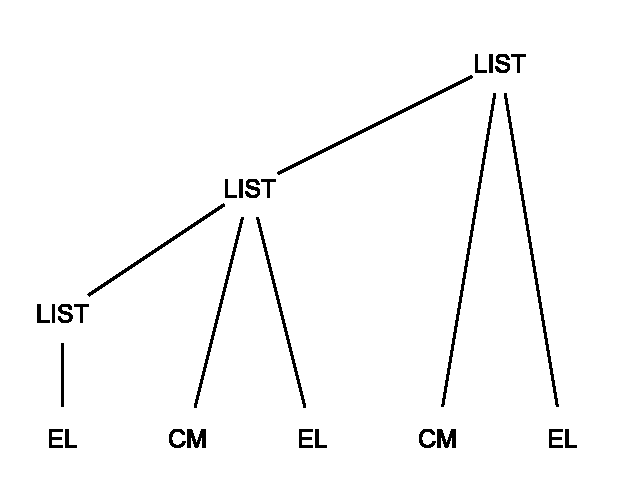
\includegraphics[width=0.5\textwidth]{img/17.pdf}}
    \end{figure}
    \item[] actions:
    \begin{table}[h]
        \centering
        \begin{tabular}{l|l}
            Action & Stack \\ \hline
             & $\varepsilon$ \\ \hline
            shift & \code{EL} \\ \hline
            reduce & \code{LIST} \\ \hline
            shift & \code{LIST CM} \\ \hline
            shift & \code{LIST CM EL} \\ \hline
            reduce & \code{LIST} \\ \hline
            shift & \code{LIST CM} \\ \hline
            shift & \code{LIST CM EL} \\ \hline
            reduce & \code{LIST} \\ \hline
        \end{tabular}
    \end{table}
\end{itemize}

\section{Introduction to CUP}
CUP is a parser generator that transforms the definition of a context-free grammar in a Java program that parses sequences of input symbols according to the grammar itself.
Besides defining syntax rules, it is possible to specify actions to be executed whenever a production is reduced.
The parser must be integrated by a scanner: some conventions simplify the integration of CUP-generated parses with JFlex-generated scanners.

\subsection{Source File Format}
A CUP source file has a syntax that is very similar to a Java program's one.
It can be ideally divided in the following sections:
\begin{enumerate}
    \item
    setup;
    \item
    terminals and non-terminals;
    \item
    precedences;
    \item
    rules.
\end{enumerate}

Comments are allowed to follow Java syntax.

\subsection{Setup Section}
This section contains all the directives needed for the parser, such as inclusion of CUP library and other libraries (\code{import java_cup.runtime.*;}).
In this section there is also a user code part, in which there are redefinitions of cup internal methods and integration with another scanner other than JFlex.

\subsection{Terminals/Non-Terminals Section}
It contains the definition of:
\begin{itemize}
    \item
    the grammar start symbol;
    \item
    terminals (passed by JFlex);
    \item
    non-terminals.
\end{itemize}

More specifically:
\begin{description}
    \item[start symbol]
    \begin{itemize}
        \item
        ``start with \code{<non_terminal_name>}'',
        \item
        it is the root of the parse tree,
        \item
        only one occurrence of this keyword is allowed;
    \end{itemize}
    \item[terminals]
    \begin{itemize}
        \item
        ``terminal \code{<term_1>}, \code{<term_2>}, \ldots'',
        \item
        \code{<term>} name contains letters, ``\_'', ``.'', and digits (the first character must be a letter),
        \item
        terminals are recognized by JFlex;
    \end{itemize}
    \item[non-terminals]
    \begin{itemize}
        \item
        ``non-terminal \code{<n_term_1>}, \code{<n_term_2>}'',
        \item
        \code{<n_term>} name contains letters, ``\_'', ``.'', and digits (the first character must be a letter).
    \end{itemize}
\end{description}

Example:
\begin{figure}[H]
    \centerline{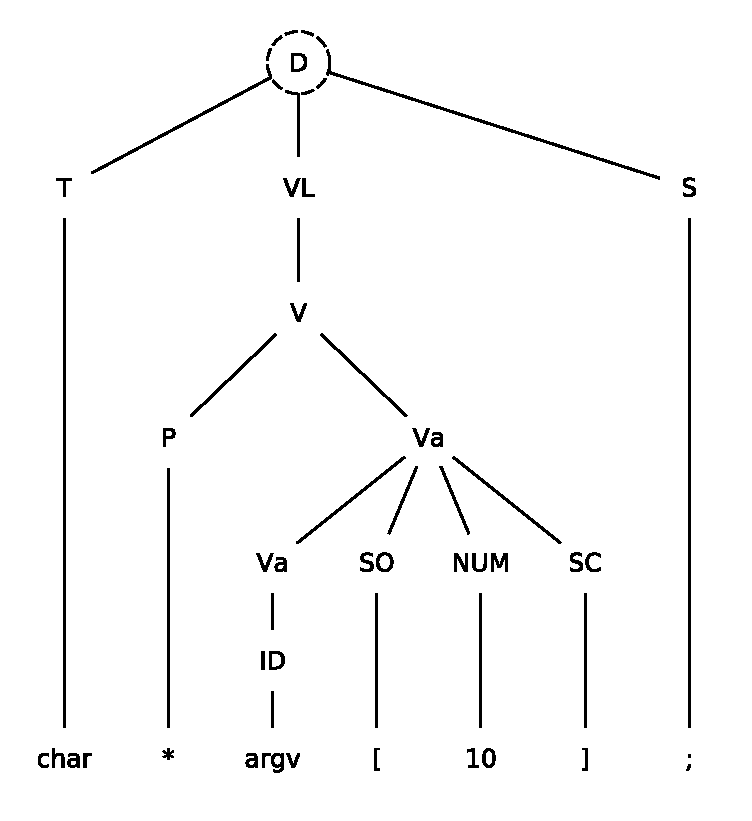
\includegraphics[width=0.5\textwidth]{img/18.pdf}}
\end{figure}
Productions (grammar rules):
\begin{align*}
    D &\to T \quad VL \quad S \\
    VL &\to V \\
    VL &\to VL \quad CM \quad V \\
    V &\to P \quad V \\
    V &\to Va \\
    Va &\to Va \quad SO \quad NUM \quad SC \\
    Va &\to ID
\end{align*}
Input string: \code{char * argv[10]}

\subsection{Rules Section}
The rules section contains one or more productions in the form of:
\begin{lstlisting}
<non_terminal> ::= right_hand_side;
\end{lstlisting}
Where \code{right_hand_side} is a sequence of zero or more symbols.

To each production, an action can be associated, which must be enclosed between ``\code{\{:}'' and ``\code{:\}}''.
Note that the action is executed right before the reduce action takes place.

Example:
\begin{lstlisting}
D ::= T VL S {:
        System.out.println("Declaration found.");
    :}
;
\end{lstlisting}

If more than one production exist for a given non-terminal, they must be grouped and separated by ``\code{\|}''.

Example:
\begin{lstlisting}
funz ::= type ID RO VL RC S {:
        System.out.println("Function prototype");
    :}
    | ::= type ID RO VL RC BO stmt_list BC {:
        System.out.println("Function");
    :}
;
\end{lstlisting}
Note that the use of the ``\code{\|}'' character generates two separated rules.
It is important to remember that the code between ``\code{\{:}'' and ``\code{:\}}'' is executed only when a given rule is matched.

Example:
\begin{lstlisting}[frame=single]
// terminals - non-terminals section
terminal T, P, ID, NUM, S, CM, SO, SC;
non terminal D, V, VL, Va;
start with D;

// rules section
D ::= T VL S;
VL ::= V | VL CM V;
V ::= P V | Va
Va ::= Va SO NUM SC | Va
\end{lstlisting}
Productions:
\begin{align*}
    D &\to T \quad VL \quad S \\
    VL &\to V \\
    VL &\to VL \quad CM \quad V \\
    V &\to P \quad V \\
    V &\to Va \\
    Va &\to Va \quad SO \quad NUM \quad SC \\
    Va &\to ID
\end{align*}

\section{Integrating JFlex and CUP}
\begin{figure}[H]
    \centerline{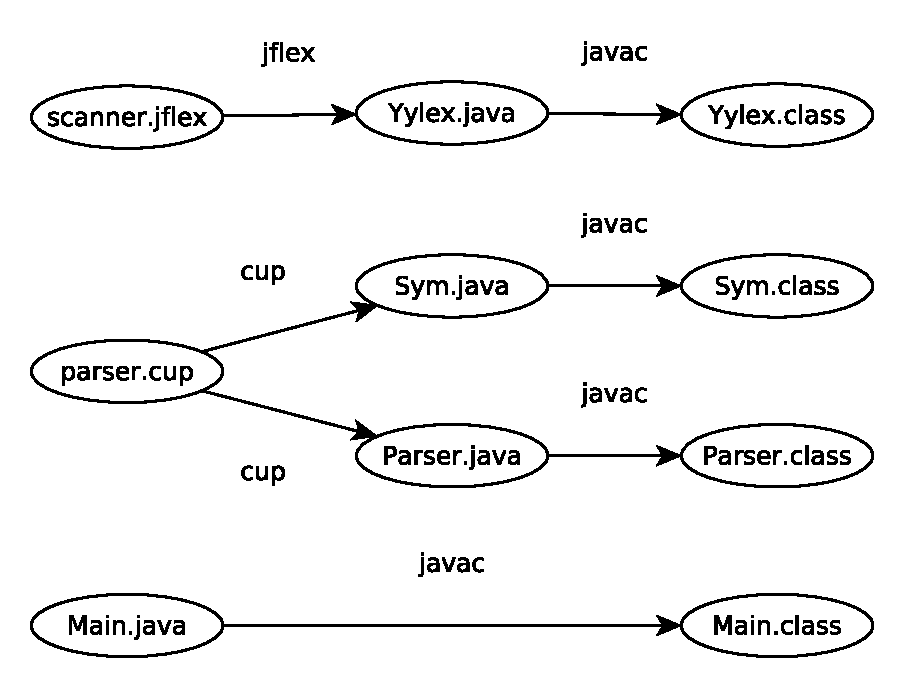
\includegraphics[width=0.6\textwidth]{img/19.pdf}}
\end{figure}

Parser and scanner must agree on the values associated to each token (terminal).
When the scanner recognizes a token, it must pass a suitable value to the parser.
This is done by means of the \emph{Symbol} class, whose constructors are:
\begin{itemize}
    \item
    \code{public Symbol (int sym_id)};
    \item
    \code{public Symbol (int sym_id, int left, int right)};
    \item
    \code{public Symbol (int sym_id, Object O)};
    \item
    \code{public Symbol (int sym_id, int left, int right, Object O)}.
\end{itemize}
The class \emph{Symbol} can be found in the CUP installation directory \code{java_cup/runtime/Symbol.java}.

When a terminal is defined by means of the terminal keyword, cup associates an integer value to that token.
This mapping is contained in the \code{Sym.java} generated by CUP during compiling processes.

Example: if in the parser the following list of terminal symbols has been declared
\begin{lstlisting}
terminal T, P, ID, NUM, PV, CM, SO, SC, S;
\end{lstlisting}
they can be used inside the scanner and passed to the parser in the following way:
\begin{lstlisting}[frame=single]
...
%%
...
%%
[a-zA-Z_][a-zA-Z0-9_]* {return new Symbol(sym.id);}
\[ {return new Symbol(sym.SO);}
\] {return new Symbol(sym.SC);}
\end{lstlisting}

\subsection{Scanner Modifications}
It includes the CUP library (\code{java.cup.runtime.*}) in the code section; it also activates CUP compatibility by means of the \code{\% cup} directive in the declaration section.

Example:
\begin{lstlisting}[frame=single]
...
%%
% cup
...
%%
[a-z]+ {return new Symbol(sym.EL);}
"," {return new Symbol(sym.CM);}
\end{lstlisting}

\subsection{The CUP Parser}
Example:
\begin{lstlisting}[frame=single]
import java_cup.runtime.*;

terminal EL, CM;
non terminal LIST, ELIST;
start with ELIST;

ELIST ::= LIST {:
        System.out.println("list found");
    :}
    | {:
        System.out.println("empty list");
    :}
;

LIST ::= LIST CM EL
;

LIST ::= EL
;
\end{lstlisting}

\subsection{Main File (\code{Main.java})}
Example:
\begin{lstlisting}[frame=single]
import java.io.*;

public class Main {
    static public void main(String argv[]) {
        try {
            // instantiate the scanner and open input file argv[0]
            Yylex L = new Yylex(new FileReader(argv[0]));
            // instantiate the parser
            Parser p = new Parser(L);
            // start the parser
            Object result = p.parse();
        } catch(Exception e) {
            e.printStackTrace();
        }
    }
}
\end{lstlisting}

\subsection{Compiling Steps}
\begin{enumerate}
    \item
    \code{jflex scanner.jflex}
    \item
    \code{java java_cup.Main parser.cup}\footnote{Note that in case of shift/reduce or reduce/reduce conflicts, the command is: \code{java java_cup.Main -expect <#conflicts> parser.cup}}
    \item
    \code{java java_cup.MainDrawTree parser.cup}\footnote{\code{MainDrawTree} is for debugging purpose.}
    \item
    \code{javac Yylex.java Sym.java Parser.java Main.java} or \code{javac *.java}\footnote{This is to compile all the files of the project.}
    \item
    \code{java Main <file>}\footnote{This is to execute the program using \code{<file>} as input.}
\end{enumerate}

\chapter{Ambiguous Grammars, Lists, Handling Syntax Errors}

\chapter{Semantic}

\chapter{Type-Checking}

\part{Exercises}

\end{document}
